\section{Gene Co-expression Networks}

    Another type of network from the field of biology are the gene co-expression networks. Each node there corresponds to a specific gene and they are connected by a link whenever there is a significant co-expression relationship between them.

    These networks are usually constructed with the help of some analysis software ot algorithm. This is because they are commonly big networks with very complex connections and unexpected clusters.

    \begin{figure}[H]
        \centering
        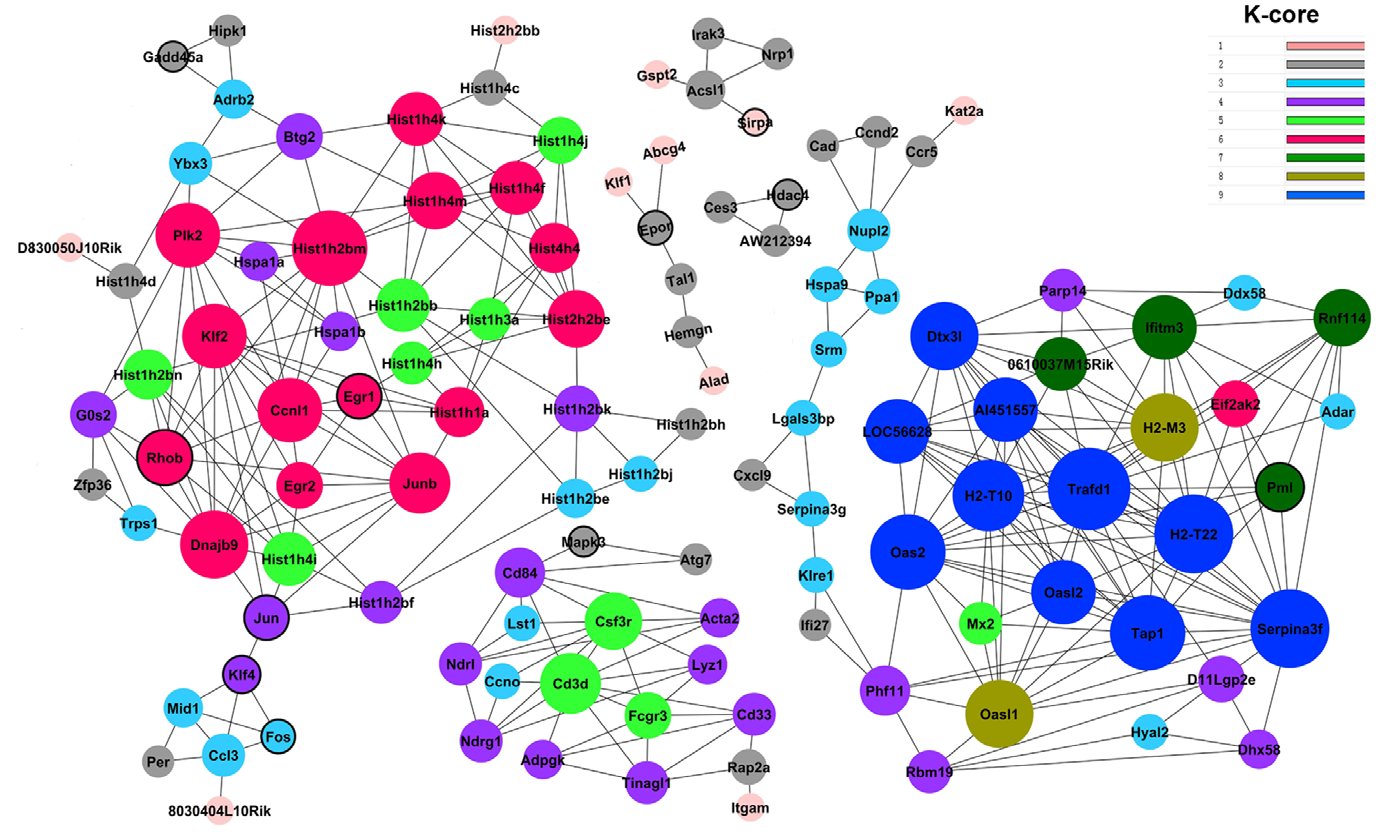
\includegraphics[width=0.9\textwidth]{images/pone-015.png}

        \caption{Co-expression of genes related to irradiation injury. From: \cite{zhang}.}
        \label{fig:gene-coexp}
    \end{figure}
